%-------------------------------------------------------------------------------
% This is a template ATLAS Paper that contains suggestions and hints on how
% to get your paper draft into a form that minimizes the amount of work needed
% to get it approved by the collaboration - assuming that the physics is OK!
%-------------------------------------------------------------------------------
\documentclass{style/atlasdoc}

% Standard packages that can and should be used in ATLAS papers
\usepackage{style/atlaspackage}
\usepackage{mathrsfs}
% Useful macros
\usepackage{style/atlasphysics}

% Use biblatex and biber for the bibliography
\usepackage[backend=biber,
	style=numeric-comp,sorting=none,block=ragged,firstinits=true]{biblatex}
\addbibresource{atlas-paper.bib}
\addbibresource{../atlas-latex.bib}

% Paths for figures
\graphicspath{{../../figures/},{figures/}}

\newcommand{\Macro}[1]{\textbackslash #1\xspace}

%-------------------------------------------------------------------------------
% Generic document information
%-------------------------------------------------------------------------------

% Set author and title for the PDF file
\hypersetup{pdftitle={ATLAS paper template},pdfauthor={ATLAS Publications Committee}}

\atlastitle{A template for ATLAS papers}

%\author{The ATLAS Collaboration}

%\draftversion{1.0}

\abstracttext{ %
  This is a template ATLAS paper. It contains the structure, style
  files and hints on how to produce a paper for which a minimum amount
  of time is necessary to spend on typographic details. This template
  can be found on the web pages of the ATLAS Publication
  Committee. You can find the technical details about to use the
  template in a separate document.
}

%-------------------------------------------------------------------------------
% Extra definitions - it is usually better to collect these in a separate file
%-------------------------------------------------------------------------------
% Shorthand for \phantom to use in tables
\newcommand*{\pho}{\phantom{0}}
\newcommand{\BibTeX}{\textsc{Bib\TeX}}

%-------------------------------------------------------------------------------
% This is where the document really begins
%-------------------------------------------------------------------------------
\begin{document}

\tableofcontents
\clearpage

%-------------------------------------------------------------------------------
\section{Front page}
\label{sec:front}
%-------------------------------------------------------------------------------

A couple of remarks about the paper front page:
\begin{itemize}

\item {\bf Title:} it should be concise, clear and descriptive, and
  should include the word ``ATLAS''.

\item {\bf Author list:} it will be provided by the Authorship
  Committee, and will be made available on their website. On the
  front page, you should name ``The ATLAS Collaboration'' as
  author.

\item {\bf Abstract:} it should also be clear, descriptive, and
  concise. It should ideally be one paragraph long, and certainly no
  more than half a page. It should stand on its own and, similarly,
  the main text of the paper should not depend on it. The abstract
  should state: what was the measurement; where was it done and with
  what dataset/luminosity; what method was used; what are the
  primary results and main conclusions.  Citations in an abstract
  should be avoided. If only Monte Carlo data are used in the
  publication, this fact should be stated explicitly in the
  abstract.  
  
\end{itemize}


%-------------------------------------------------------------------------------
\section{Introduction}
\label{sec:intro}
%-------------------------------------------------------------------------------

The introduction should be fairly brief, not more than one page.
State the measurement being made, motivate its importance
experimentally and theoretically. Include a summary of what is known
to date about this measurement. Give a brief outline for the rest of
the paper.

Your first action before embarking on writing a paper should be to
read the ATLAS Publication Policy~\cite{publication-policy}, available
from the web pages of the Publication Committee. Chapter 3 of this
document details the refereeing and approval procedures that you will
need to follow; Chapter 4 gives information on the style.

At some point during the writing of an ATLAS paper, 
you should decide what journal it will be submitted to.
Please keep in mind that each journal makes specific demands on length and style.
Most journals use regular capitalisation for titles 
(i.e.\ capitalise the first word and all proper nouns, 
e.g.\ ``The search for large extra dimensions''). 
The notable exception is Physical Review Letters, which capitalizes the
first word and all other important words,
e.g.\ ``The Search for Large Extra Dimensions''.

The \LaTeX{} file and Postscript versions of this template can be
found on the web pages of the ATLAS Publication Committee. Example
macros for figures can be found there as well.  Comments and/or
suggestions on improvements to this template are very welcome and
should be given to the Publication Committee.

The \texttt{atlasphysics.sty} style file contains a set of particles,
reactions, etc.\ that may be useful. For example, the missing-$E_{\text{T}}$
symbol (\met{}) is defined there. 
A separate document~\cite{atlas-physics}
contains a list of the commands in \texttt{atlasphysics.sty}.

This paper template has been tested using \LaTeX{}2e.  You should get
this version automatically. If you have problems check which \LaTeX{}
version you are running.


%-------------------------------------------------------------------------------
\section{Theory}
\label{sec:theory}
%-------------------------------------------------------------------------------

Give here a brief explanation of the theory relevant for this paper,
with proper referencing. Use, for example,
\verb|\cite{Glashow:1961tr,Weinberg:1967tq,sm_salam}| to cite the
Standard Model~\cite{Glashow:1961tr,Weinberg:1967tq,sm_salam}.

Define important quantities that will be used later.
State how the measurement of interest is actually performed, and how parameters are
extracted from the data.  
If quantities are extracted with a fit to the data, describe the fit procedure.
If the explanation needs to be a bit longer, a separate section may be appropriate.


%-------------------------------------------------------------------------------
\section{Experimental setup}
\label{sec:atlas}
%-------------------------------------------------------------------------------

The Publication Committee provides a standard texts giving examples
for description of the ATLAS detector, and the appropriate references.
This text is included in the paper template provided with this package.
If necessary for your analysis, describe a subdetector in more detail.

The section on the experimental setup should also describe the dataset:
when were the data taken, under what specialcircumstances (if any),
and what was the integrated luminosity.

Examples of descriptions can be found below.

% Footnote with ATLAS coordinate system
\newcommand{\AtlasCoordFootnote}{%
ATLAS uses a right-handed coordinate system with its origin at the nominal interaction point (IP)
in the centre of the detector and the $z$-axis along the beam pipe.
The $x$-axis points from the IP to the centre of the LHC ring,
and the $y$-axis points upwards.
Cylindrical coordinates $(r,\phi)$ are used in the transverse plane, 
$\phi$ being the azimuthal angle around the beam pipe.
The pseudorapidity is defined in terms of the polar angle $\theta$ as $\eta = -\ln \tan(\theta/2)$.
Angular distance is measured in units of $\Delta R \equiv \sqrt{\Delta\eta^{2} + \Delta\phi^{2}}$.}

%-------------------------------------------------------------------------------
\subsection{ATLAS detector}
\label{sec:atlas1}
%-------------------------------------------------------------------------------

The ATLAS experiment~\cite{atlas-detector} at the LHC is a multi-purpose particle detector
with a forward-backward symmetric cylindrical geometry and a near $4\pi$ coverage in 
solid angle\footnote{\AtlasCoordFootnote}.
It consists of an inner tracking detector surrounded by a thin superconducting solenoid
providing a \SI{2}{\tesla} axial magnetic field, electromagnetic and hadron calorimeters, and a muon spectrometer.
The inner tracking detector covers the pseudorapidity range $|\eta| < 2.5$.
It consists of silicon pixel, silicon micro-strip, and transition radiation tracking detectors.
Lead/liquid-argon (LAr) sampling calorimeters provide electromagnetic (EM) energy measurements
with high granularity.
A hadron (iron/scintillator-tile) calorimeter covers the central pseudorapidity range ($|\eta| < 1.7$).
The end-cap and forward regions are instrumented with LAr calorimeters
for both EM and hadronic energy measurements up to $|\eta| = 4.9$.
The muon spectrometer surrounds the calorimeters and is based on
three large air-core toroid superconducting magnets with eight coils each.
Its bending power is in the range from \num{2.0} to \SI{7.5}{\tesla\metre}.
It includes a system of precision tracking chambers and fast detectors for triggering.
A three-level trigger system is used to select events.
The first-level trigger is implemented in hardware and uses a subset of the detector information
to reduce the accepted rate to at most \SI{75}{\kilo\hertz}.
This is followed by two software-based trigger levels that
together reduce the accepted event rate to \SI{400}{\hertz} on average
depending on the data-taking conditions during 2012.


%-------------------------------------------------------------------------------
\subsection{ATLAS coordinate system footnote}
\label{sec:coord}
%-------------------------------------------------------------------------------



%-------------------------------------------------------------------------------
\section{Monte Carlo}
\label{sec:MC}
%-------------------------------------------------------------------------------

Any Monte Carlo programs used must be clearly stated with full version
number. A brief description of the program is useful but not necessary
unless a less well known program is used.  Any corrections or special
parameter settings must be clearly explained.  The statistics should
be given if the amount used results in a non-negligible uncertainty.


%-------------------------------------------------------------------------------
\section{Event selection}
\label{sec:selection}
%-------------------------------------------------------------------------------

List the trigger and offline selection criteria, give the obtained
statistics.


%-------------------------------------------------------------------------------
\section{Data characteristics}
\label{sec:control}
%-------------------------------------------------------------------------------

Discuss here the characteristics of the data, in terms of
primary quantities and backgrounds.


%-------------------------------------------------------------------------------
\section{Systematic uncertainties}
\label{sec:syst}
%-------------------------------------------------------------------------------

Give a detailed list of systematic uncertainties, the method
by which they were obtained, and a justification of the resulting
values.
%
Use ``systematic uncertainty'' instead of ``systematic errors''.
The latter sounds as if you have made a mistake systematically.


%-------------------------------------------------------------------------------
\section{Results}
\label{sec:result}
%-------------------------------------------------------------------------------

State the results without interpretations.


%-------------------------------------------------------------------------------
\section{Discussion}
\label{sec:discussion}
%-------------------------------------------------------------------------------

Put the results into the context of the theory or a model.
%
If the results lead to exclusion plots, make sure that it is clear 
which region on the plot is excluded.


%-------------------------------------------------------------------------------
\section{Summary and conclusion}
\label{sec:summary}
%-------------------------------------------------------------------------------

Reiterate the main points of the paper and the primary results and
conclusions.

Note that many readers look mostly at the title, abstract and
conclusion. The conclusion should be interesting enough to
make them want to read the whole paper.
It is not good style to just repeat the abstract.

If your paper is short and only has one result quoted at the end of
the paper, then you should consider whether conclusions are
necessary. 

Try not to end your conclusions with a sentence such as
``All the results in this paper are in good agreement with the
Standard Model, the current world average and recent
measurements by other experiments''. This might lead a referee
(internal or external) to wonder why it is worth publishing this
paper!

Note that all figures and tables should be output before the start of the
``Summary and conclusion''. 


%-------------------------------------------------------------------------------
\section*{Acknowledgements}
\label{sec:acknowldge}
%-------------------------------------------------------------------------------

A standard template for the acknowledgements is available on the
web pages of the Publication Committee.
See reference~\cite{publication-policy} for the URL. 

The acknowledgements should be in an unnumbered section.


%-------------------------------------------------------------------------------
% Bibliography
%-------------------------------------------------------------------------------
\printbibliography
% This document uses biblatext and bib to process the bibliography.
% If you want to use BibTeX you need to use the syntax below.
% \bibliographystyle{../atlasBibStyleWoTitle}
% \bibliography{atlas-paper}


%-------------------------------------------------------------------------------
\newpage
\appendix
\part*{Appendices}
\addcontentsline{toc}{part}{Appendices}
%-------------------------------------------------------------------------------

In general, you use the appendices to include all the technical details of your work
that are relevant for the ATLAS Collaboration only (e.g.\ dataset details, software release used).
In an ATLAS paper auxiliary plots and tables that are supposed to be made public 
should be collected in an appendix.

Use the following commands to start the Appendices section:
\begin{verbatim}
   \newpage
   \appendix
   \part*{Appendices}
   \addcontentsline{toc}{part}{Appendices}
\end{verbatim}

In this document the appendices contain some general remarks on the style to use in ATLAS papers
and some technical aspects on how to implement the style.
More details on how to use the ATLAS \LaTeX\ templates to help you follow 
these recommendations can be found in other documents:
\begin{itemize}
\item ATLAS style guide~\cite{atlas-style}.
\item ATLAS \LaTeX\ guide~\cite{atlas-latex};
\item ATLAS \BibTeX\ guide~\cite{atlas-bibtex};
\item ATLAS physics symbols~\cite{atlas-physics}.
\item Rounding in ATLAS~\cite{atlas-rounding};
\end{itemize}

%-------------------------------------------------------------------------------
\section{General Style}
\label{sec:english}
%-------------------------------------------------------------------------------

We recommend the use of British English. However, whatever you decide
to choose, be consistent throughout the paper. For much more detailed
information on writing, spelling and typographic style, etc. please
see the ATLAS Style Guide~\cite{atlas-style}. 
The ATLAS Glossary~\cite{atlas-glossary} contains a list of ATLAS detector acronyms.


%-------------------------------------------------------------------------------
\subsection{Emphasis}
\label{sec:emphasis}
%-------------------------------------------------------------------------------

Use italics for emphasis sparingly: too many italicised words defeat
their purpose. When you do italicise a word, really italicise it: do
not use math mode! Note the difference between \emph{per se}
(\verb|\emph{per se}|) and $per se$ (\verb+$per se$+). Abbreviations
like i.e., e.g., etc., and et al.\ should \emph{not} be italicised!
For program names we recommend to use small capitals:
\verb|\textsc{Pythia}}| produces \textsc{Pythia}.


%-------------------------------------------------------------------------------
\section{Tables}
\label{sec:table}
%-------------------------------------------------------------------------------

All tables appearing in the paper must be mentioned in the text. The
tables should appear in the same order as mentioned in the text. Do
not abbreviate the word ``Table''. Capitalise the first word of any
row or column heading. Label all rows/columns, including units if
appropriate. Units are given in brackets, e.g.\ ``Energy [\si{\GeV}]''.
Horizontal and vertical lines should be kept to a minumum and only used 
as necessary to make the table entries clear.
The table caption appears below the table.  
Any symbols/variables used in the table must be defined in the
caption.  Always use labels to refer to tables and figures. Note that
the label must be included in the body of the caption.

If table entries include uncertainties, the entries should be aligned
on the ``$\pm$'' sign. Numbers look best when aligned on the decimal
point. Otherwise, column entries should be left-aligned.
Table~\ref{tab:example1} shows the use of $\pm$ as the intercolumn
character for alignment. An alternative, as shown in
Table~\ref{tab:example2}, is to use \verb+\phantom+ to put in extra
space equal to the width of a number if you have different numbers of
decimal places in the table.
The note on rounding~\cite{atlas-rounding} contains more examples on how to format tables.

The \texttt{booktabs} package provides the macros 
\Macro{toprule}, \Macro{midrule}, \Macro{bottomrule} which are to be preferred over \Macro{hline},
as, among other things, they introduce some extra spacing around the lines, which is useful.

\begin{table}[htbp]
  \centering
  \begin{tabular}{l S[table-format=2.1]@{$\;\pm\;$}S[table-format=1.1]@{\,}s
  	S[table-format=3.1]@{\,}s}
    \toprule
    Category            & \multicolumn{3}{c}{$\mu$}&\multicolumn{2}{c}{$e$}\\ 
    \midrule
    $b \to \ell$        &     65.2 & 0.4 & \%   &  79.3 & \% \\
    $b \to c \to \ell$  &      7.8 & 0.3 & \%   &   5.4 & \% \\
    Total               &     73.0 & 0.2 & \%   &   9.1 & \% \\ 
    \bottomrule
  \end{tabular}
  \caption[Monte Carlo purities in the single lepton sample]{%
  	Monte Carlo estimates of the fraction of each process in the single
    lepton data sample. This table uses ``S'' format from \texttt{siunitx} and
    ``\texttt{$\,\pm$\,}'' as the intercolumn separator.}
  \label{tab:example1}
\end{table}


\begin{table}[htbp]
  \centering
  \begin{tabular}{lcc}
    \toprule
    Category            & \multicolumn{1}{c}{$\mu$}&\multicolumn{1}{c}{$e$}\\ 
    \midrule
    $b \to \ell$        & $    65.2 \pm 0.4\,\%$   &     79.3\,\% \\
    $b \to c \to \ell$  & $\pho 7.8 \pm 0.3\,\%$   & \pho 5.4\,\% \\
    Total               & $    73.0 \pm 0.2\,\%$   & \pho 9.1\,\% \\ 
    \bottomrule
  \end{tabular}
  \caption{Monte Carlo estimates of the fraction of each process in
    the single lepton data sample. 
    This table uses \texttt{\textbackslash phantom}.}
  \label{tab:example2}
\end{table}


%-------------------------------------------------------------------------------
\section{Figures}
\label{sec:figure}
%-------------------------------------------------------------------------------

The Publication Committee has a root macro to create figures in
ATLAS style, it can be found on the Publication Committee web pages.
Use this style consistently throughout the paper.
An example figure can be seen in Figure~\ref{fig:example}. 

\begin{figure}[htbp]
  \centering
  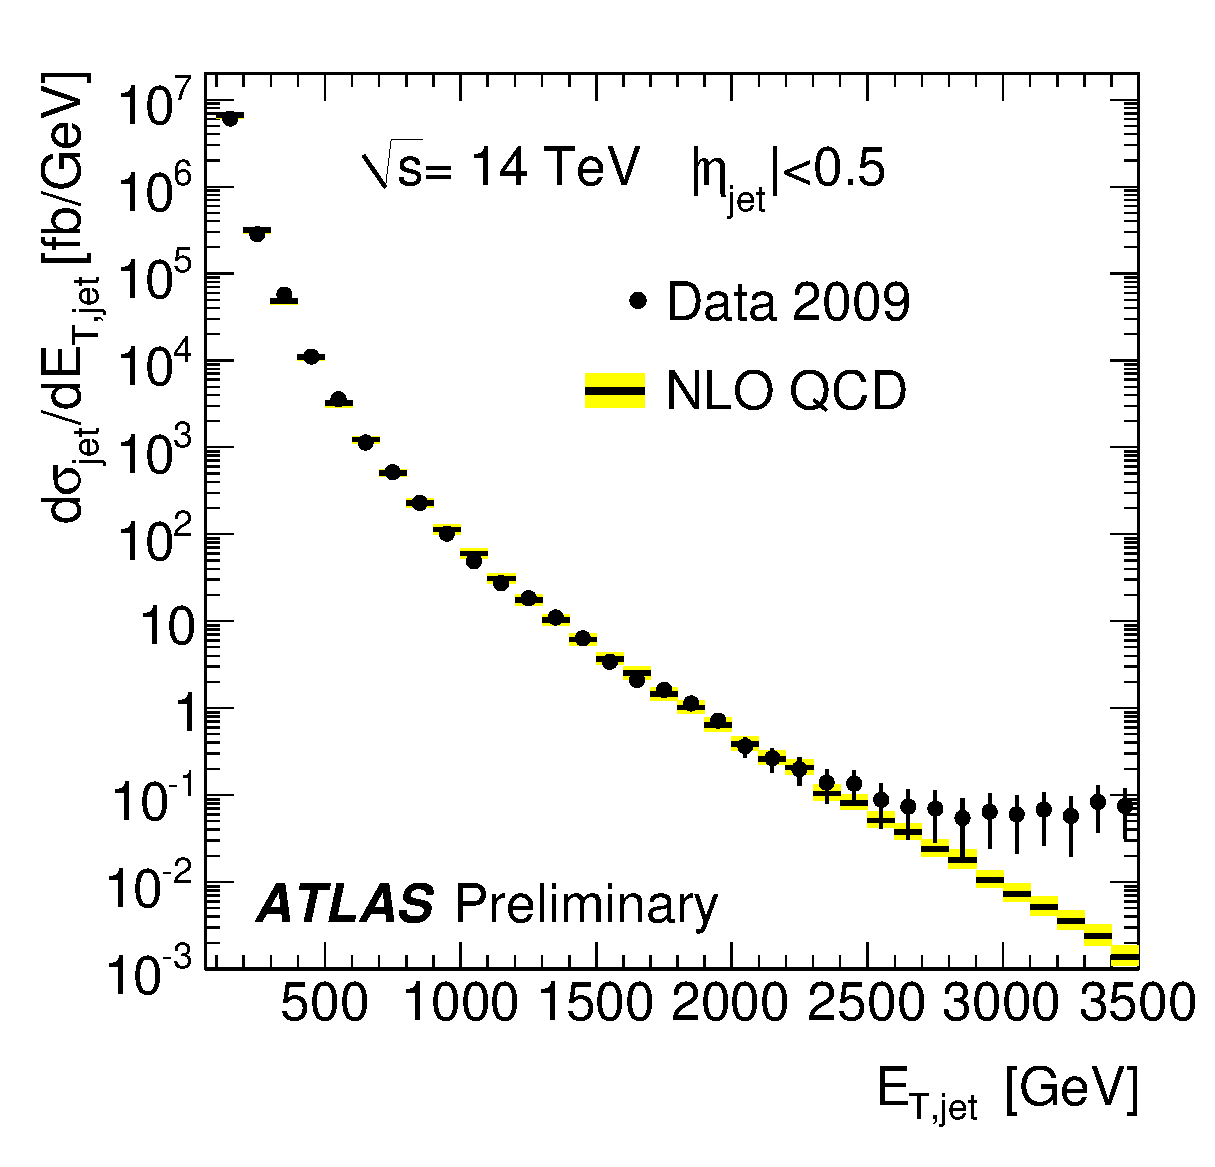
\includegraphics[width=\columnwidth]{AtlasExample}
  \caption{An example ATLAS figure.}
  \label{fig:example}
\end{figure}

Figures should be always made available in both \texttt{eps} (or \texttt{pdf}) and 
\texttt{png} format. Additionally, a {\tt pdf} version of the plots can be
useful in case \verb|pdflatex| is used to produce a publication.
%Colour versions are appropriate for talks, and black-and-white
%versions are necessary for the publication itself.

All figures appearing in the paper must be mentioned in the text.
The figures should appear in the same order as mentioned in the text.
At the beginning of a sentence, use the full word ``Figure''.
Within a sentence, the abbreviation ``Fig.'' may be used.
If a figure appears in two or more parts, refer to it as
``Fig. 1(a)'' and ``Fig. 1(b)''. Both ``(a)'' and ``(b)'' should
appear in the text, in the figure, and in the caption.
The word ``ATLAS'' (or ``ATLAS Preliminary'', if appropriate) should
appear prominently somewhere in the figure. This becomes important when
the figure is copied and shown out of context. If appropriate, it
is useful to include information about the luminosity corresponding
to a figure.

All axes must be labeled, including units (i.e. ``Energy [\gev]'').
The vertical axis units should specify the bin width, unless
arbitrarily normalized. A legend box explaining all plotting symbols
must appear somewhere in the figure.

The caption should be placed below the figure.  All lines, all
plotting symbols, and all variables used in the figure must be defined
in the caption. Do not refer to any characteristic that is not
distinguishable in black-and-white.  If relevant, the normalization
method of the plot should be specified.

A figure with subfigures can be made as shown in the example of
Figure~\ref{fig:subfigexample}.

\begin{figure}
  \centering
  \subfigure[One subfigure example]{
    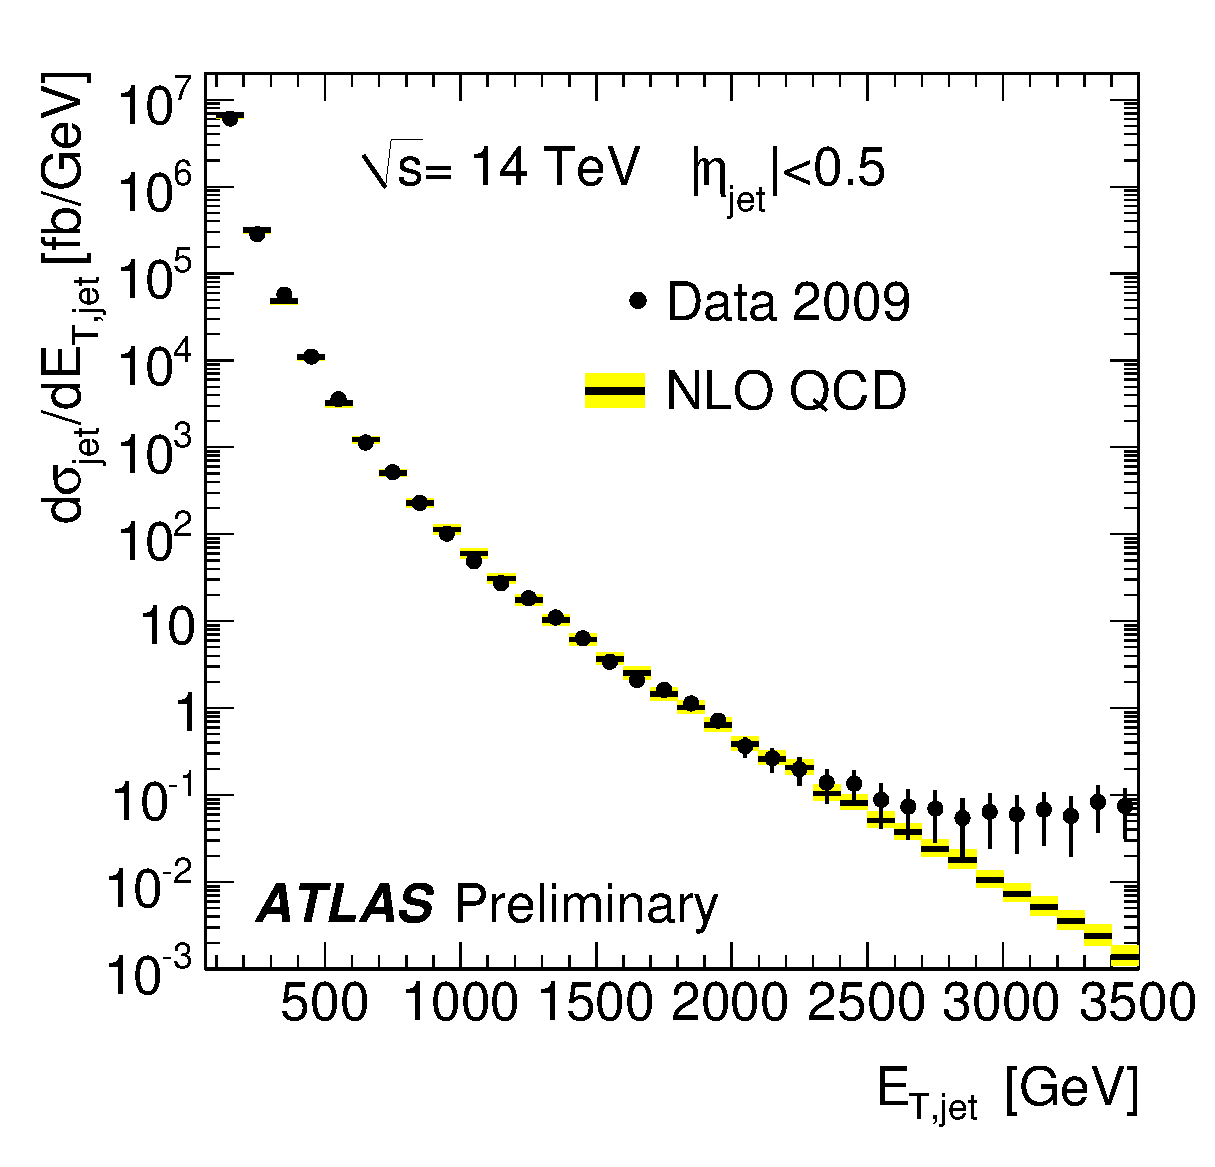
\includegraphics[width=0.55\textwidth]{AtlasExample}
    \label{fig:SubfigureExample1}
  }
  \subfigure[Another subfigure example]{
    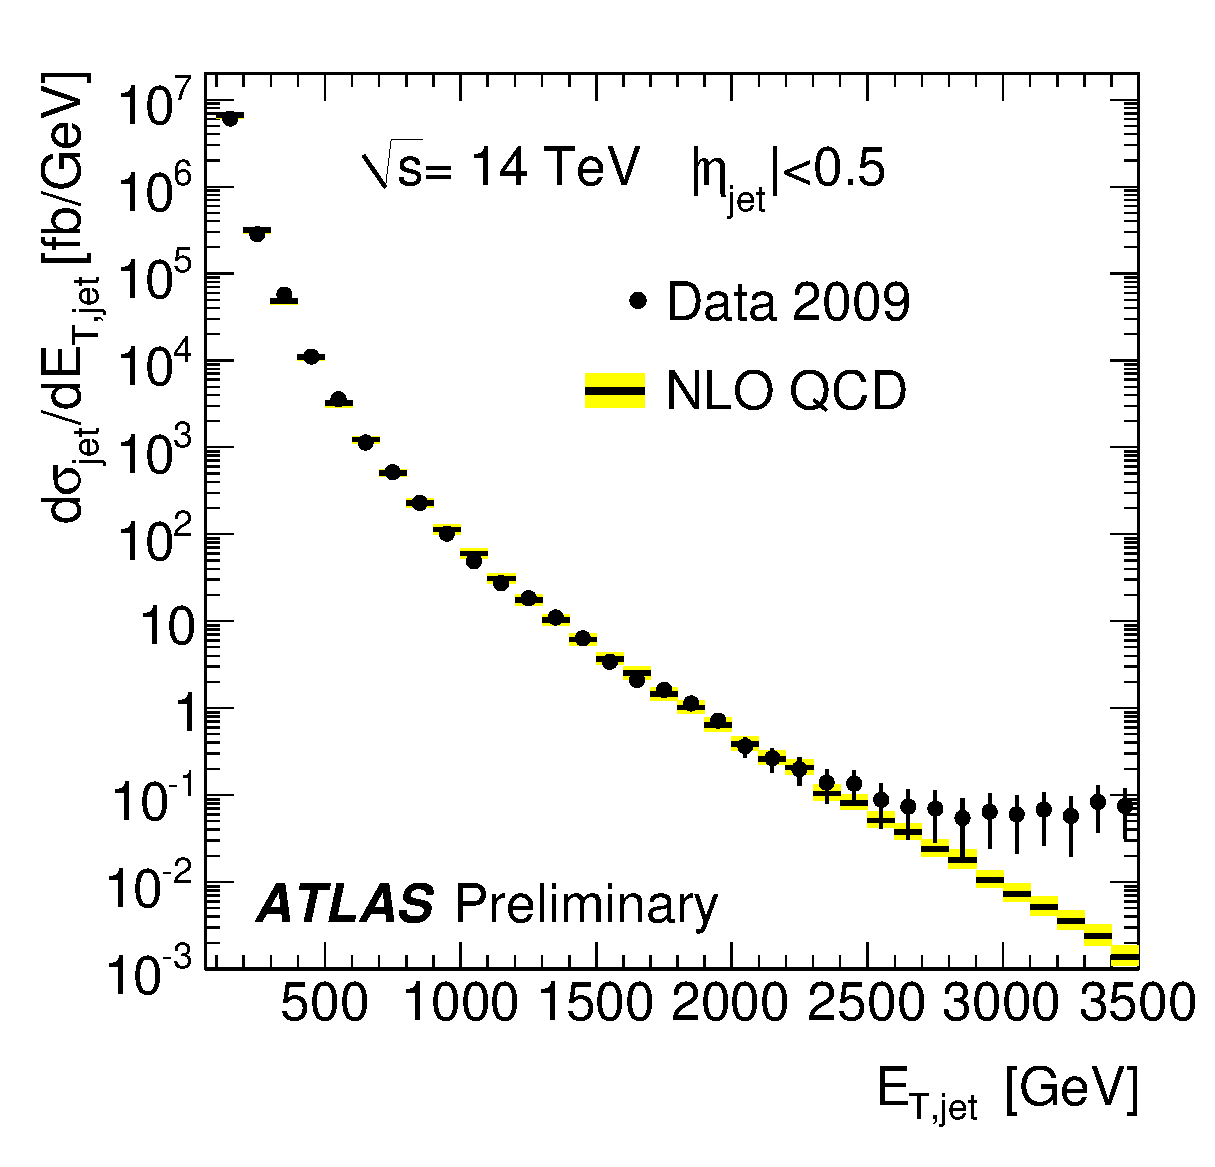
\includegraphics[width= 0.55\textwidth]{AtlasExample}
    \label{fig:SubfigureExample2}
  }
  \caption{Subfigure example (\ref{fig:SubfigureExample1}) and
    (\ref{fig:SubfigureExample2}).}
  \label{fig:subfigexample}
\end{figure}


%-------------------------------------------------------------------------------
\section{References}
\label{sec:refs}
%-------------------------------------------------------------------------------

Only cite permanent, publicly available, or ATLAS approved references.
Private references, not available to the general public, should be
avoided. Caution should be used when referring to ATLAS notes.
Only reference approved notes. Do not reference COM or INT notes,
as these are not available outside ATLAS.

Whenever possible, cite the article's journal rather than its preprint number. 
If possible, the arXiv number should be given in addition.
Always double check references when copying them from another source.

Referencing styles are journal-dependent. See the ATLAS Publication
Policy document for more information.

Use \BibTeX{} for the references. Although it often
appears harder to use at the beginning, it means that the number of
typos should be reduced significantly and the format of the references
will be correct, without you having to worry about formatting it. In
addition the order of the references is automatically correct.

One or more files with the extension \texttt{.bib} 
(in this example: \texttt{atlas-paper.bib}) should contain all the references. 
The files may also contain references that you do not use, so they may act like a
library of references. 
The typical compilation cycle when using \BibTeX{} looks like the following:
%
\begin{verbatim}
  (pdf)latex instructions
  bibtex instructions
  (pdf)latex instructions
  (pdf)latex instructions
\end{verbatim}
%
\BibTeX{} will create a file with the extension \texttt{.bbl}, which will
contain the actual references used, and \LaTeX{} will then take care
to include them in your paper. Note that only after the third run of
\LaTeX{} will all references be correct. Unless you change a reference
you do not have to do the \texttt{bibtex} step again.

Two \BibTeX{} style files 
(\texttt{style/atlasBibStyleWoTitle.bst} and \texttt{style/atlasBibStyleWoTitle.bst})
are provided with the ATLAS \LaTeX\ package. 
You can use one of them in your text source file as follows:
%
\begin{verbatim}
  \bibliographystyle{atlasBibStyleWoTitle}
  \bibliography{atlas-paper}
\end{verbatim}

Note that \texttt{biblatex} is a more modern replacement for \BibTeX\ that has a number of advantages.
If you want to use this package, you should include commands like:
%
\begin{verbatim}
  \usepackage[backend=biber,
	  style=numeric-comp,sorting=none,block=ragged,firstinits=true]{biblatex}
  \addbibresource{atlas-paper.bib}
\end{verbatim}
%
in the preamble of our document.
The include the command:
%
\begin{verbatim}
  \printbibliography
\end{verbatim}
%
where the bibliography should get printed.
Use the command \texttt{biber} instead of \texttt{bibtex} to process the \texttt{.bib} files.

For further information on \BibTeX{} and on the standard ATLAS style for referencing, 
see the ``ATLAS \BibTeX Guide''~\cite{atlas-bibtex}.


%-------------------------------------------------------------------------------
\section{The \texttt{atlasdoc} class}
\label{app:atlasdoc}
%-------------------------------------------------------------------------------

This paper has been typeset using the \texttt{atlasdoc.cls} class.
This class implements the ATLAS template and can be used for papers, preprints,
notes. The class is available from the web pages of the
Publication Committee and from SVN.
It also contains this instruction paper and the related files.

Details on how to use the templates can be found in a separate document
\texttt{atlas-latex.pdf}~\cite{atlas-latex}.

The style file \texttt{atlasphysics.sty} defines a lot of useful
macros for particles and more. See the separate document
\texttt{atlas-physics.pdf}~\cite{atlas-physics} for details.


%-------------------------------------------------------------------------------
\section{Remarks on units and symbols}
%-------------------------------------------------------------------------------

It is highly recommended to use a units package to format your units properly.
The package \texttt{siunitx} works very well and is the package of choice.
Alternatives include \texttt{units} and \texttt{hepunits},
which is based on \texttt{SIunits}.

If you use a units package, it automatically set SI units in roman-type font
and leaves a small space between
the value and the units (e.g.\ \SI{12}{\mm}). 
In addition, it makessure they end up
always together on the same line. \verb|\SI{12}{\mm}|.
Natural units, where $c=\hbar=1$, should be used for all
ATLAS publications. Masses are therefore in \si{\GeV}, not \si[per-mode=symbol]{\GeV\per\clight}.

Use math mode for all symbols (e.g. use $c$ (\verb|$c$|) rather than simply c). 
Momentum should be in lower case \verb+$p$+. 
Transverse momentum is a lower case $p$ with an upper case roman $\text{T}$ subscript: 
\verb|\pT| produces \pT.
Energy is an upper case \verb+$E$+, \verb+\ET+ produces \ET.  
Use \verb|\mathscr| mode for luminosity $\mathscr{L}$ $\mathcal{L}$ or aplanarity
$\mathscr{A}$ $\mathcal{A}$, including the package \verb|mathrsfs.sty|.

Trigonometric functions should be in roman type. Natural logarithm
should be ln and log base 10 is log.  When in math mode, use
\verb+$\ln$, $\sin$,+ etc. We recommend to specify the base of the
logarithm: \verb+$\log_{10}$+.

If your note makes use of cones, for example cone-jets, explain that
these cones are constructed in $\eta$-$\phi$ space, and define $\eta$.

Add the word \emph{events} as the unit when quoting the number of
events: ``The resulting background is $4.0 \pm 1.3$ events.''.  The
number of expected events should be written as $N_{\rm pred}$ rather
than $N_{\rm exp}$, since the latter could also mean experimental.

For particle names and symbols, ATLAS uses the standards of the
Particle Data Book. Intermediate vector bosons should be called
\emph{W boson(s)} and \emph{Z boson(s)}, not just \emph{W's} or
\emph{Ws}. The Z boson should not have a superscript of 0. W without
the word boson attached may be used in \emph{W pair production}, and
similar phrases.  Other particle names should be spelled out when used
in a sentence: muon(s), electron(s), tau lepton(s). \emph{Top quark}
should be used instead of \emph{top} in most places: say ``top quark
mass'' instead of ``top mass''.  Top quark and bottom quark may be
shortened to $t$ quark and $b$ quark. The neutrino
symbol $\nu$ should not have any subscripts, unless necessary for
understanding. For the \Jpsi{} use the command \verb+\Jpsi+ from {\tt
atlasphysics.sty}: it will produce a lower case $\psi$.

When in doubt, use the PDG style.

\end{document}
